\documentclass{article}
\usepackage{authblk}
\usepackage{graphicx}
\usepackage{amsmath}

\usepackage[left=2.5cm,top=3cm,right=2.5cm,bottom=3cm,bindingoffset=0.5cm]{geometry}
\title{Boron erosion on a tungsten substrate using the TOMAS ICWC antenna}
\author[1,2]{A. Adriaens}
\affil[1]{Laboratory for Plasma Physics LPP-ERM/KMS, Brussels, Belgium}
\affil[2]{Department of Applied Physics, Ghent University, Belgium}
\date{}

\setcounter{Maxaffil}{0}
\renewcommand\Affilfont{\itshape\small}

\begin{document}
\maketitle
\section{Introduction}
\subsection{Boronization}
The interior of a fusion reactor is extremely hostile, as such a refractory material
needs to be chosen for plasma facing components (PFC), tungsten is increasingly
favoured over other materials due to its unique combination of properties such
as low erosion rate, low tritium retention and resistance to heat-induced
stress \cite{PHILIPPS2011S2}\cite{Tungsten}.  But there are two big drawbacks to
using tungsten as a PFC: As it has a very high Z-value, if it does get
sputtered, high amounts of radiation loss may occur due to brehmstrahlung
\cite{JWinter_1996} and second it's a very bad oxygen getterer which is the most deleterious
of all impurities encountered in a fusion device. We can get the "best of both worlds" by
coating our tungsten with a small ($<$100nm) layer of a low Z-material.
Previously Beryllium was considered the main candidate but due to it's high
toxicity and difficulty of handling the now most favored candidate is boron.
Boronization (the deposition of a thin film of boron) has a proven track record
of causing better confinement times and ELM (Edge Localized Mode) control
\cite{ASDEXBoronisation}\cite{DIII-DBoronisation}\cite{EASTBoronisation}\cite{TEXTORBoronisation}.
There is however, at the time of writing, no direct research to the rapidity of
Boron erosion under wall conditioning techniques such as ICWC, that gap is what
this paper tries to fill.
\subsection{Experimental setup}
\begin{figure}[ht]
    \centering
    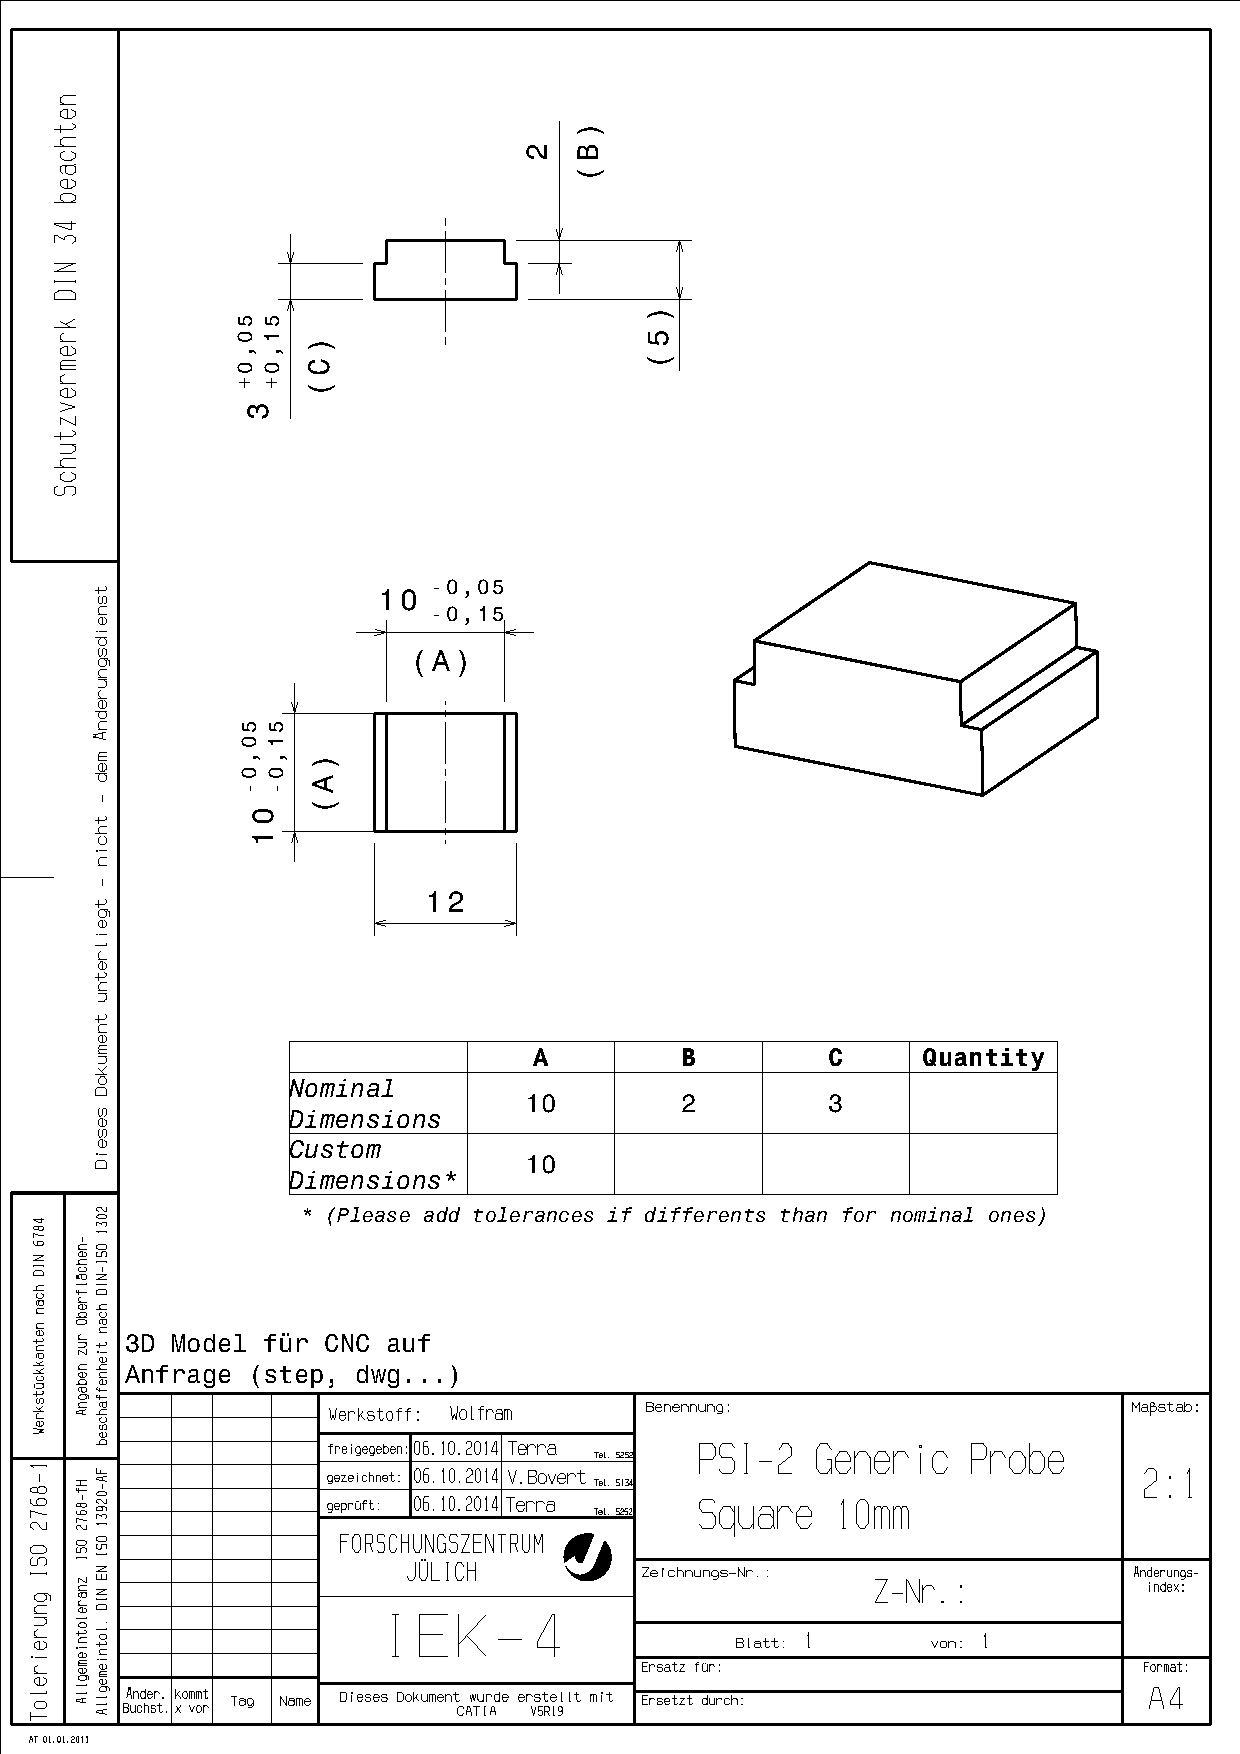
\includegraphics[height=0.33\textwidth]{figures/Sample.pdf}
    \includegraphics[height=0.33\textwidth]{figures/mask.pdf}
    \caption{The mask (right figure) is made out of tungsten and can contain 8 samples (left figure), 
    the 10x10mm top of the samples are coated with boron and attached in the mask such that it is facing towards    the plasma in the vessel}
    \label{fig:samples+mask}
\end{figure}
One may analyse boron-tungsten erosion by using neutral and ion beams,
mimicking ICWC, the obvious advantage being that the experiment is simpler with
easily chosen and controlled parameters.  But the disadvantage is that co-operative effects,
which may occur only when a plasma is present, will not be observed
\cite{McCRACKEN}. The TOMAS machine \cite{TOMAS} will be used as it is capable
of forming a full plasma during an ICRH discharge and thus introducing these
co-operative effects.  It is equiped with a monopole ICWC antenna which will be
set to operate at 50MHz, closely mimicking the 53MHz that will likely be used
at ITER.  The mask containing the samples (see figure \ref{fig:samples+mask})
is mounted on a movable arm which we'll position on top of the vessel.  
We'll modify the pressure in such a way that the
neutrals pressure (i.e the observed pressure during the discharge) is $10^{-5}$
mbar, closely mimicking what was the case in JET and will likely be the case in
ITER \cite{DOUAI}.
\section{Erosion estimation using neutrals}
\subsection{Explanation of the theory}
Sputtering due to ICWC is said to be mainly caused by high energy neutrals (citation needed), as such 
our main estimate of sputtering will be the neutrals we measure in the vessel
using the ToF-NPA, as mentioned in Daniels work (citation needed), for our experimental setup.
\noindent
\begin{figure}[ht]
    \centering
    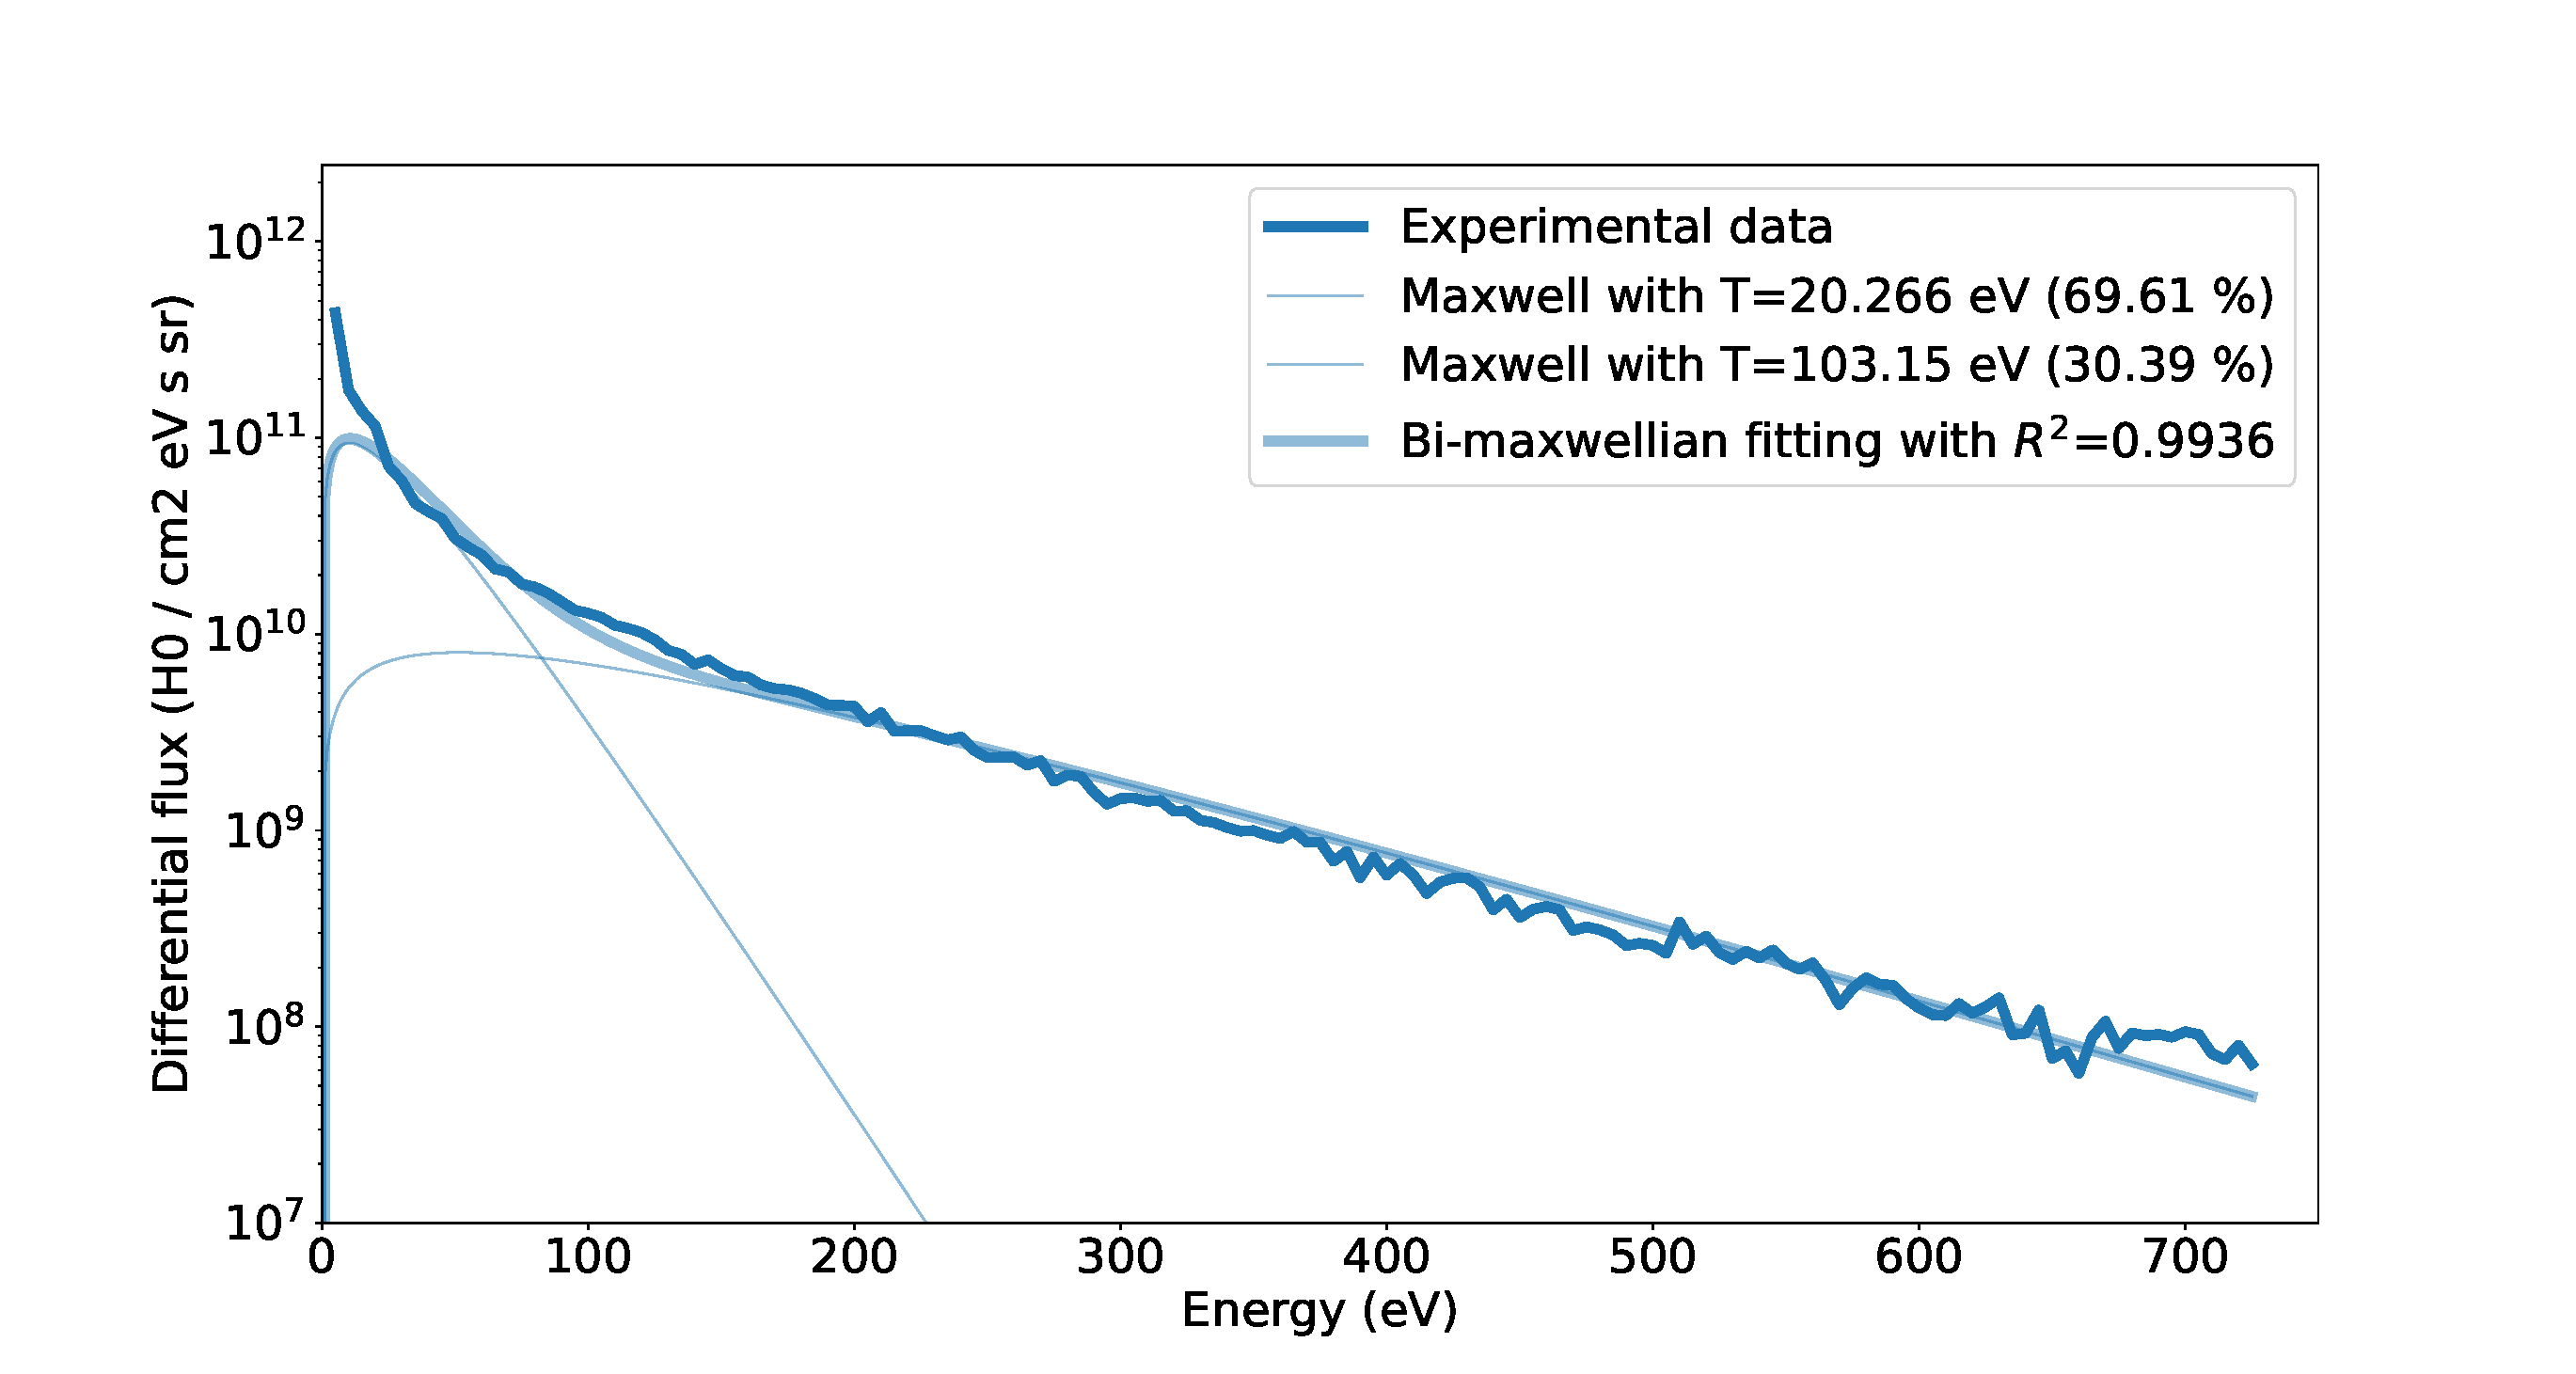
\includegraphics[width=0.7\textwidth]{figures/NPA_example.pdf}
    \caption{The assumption behind the bi-maxwellian distribution is that we have
    the conversion of heated ions to neutrals resulting in the high temperature
    maxwellian, and ions indirectly heating neutrals due to collisions, resulting
    in the low temperature maxwellian. There is, however, no verification of this
    notion yet. Note that the $R^2$ of the fitting is
    defined with the logarithmic difference to better emphesize the shape.}
    \label{fig:examplemeasurement}
\end{figure}\\
An example measurement made with the NPA is shown in figure
\ref{fig:examplemeasurement}. As the data is expressed as differential flux,
it lends itself to be easily manipulated into other quantities. One such manipulation
is using the following formula to transform it into an ersoion rate:
\begin{equation}
    S = \frac{2\pi}{N} \int_E Y(E)\mathcal{F} (E) \text{dE}
    \label{eqn:ErosionRateFormal}
\end{equation}
With $Y(E)$ the yield of the neutrals on the material (i.e how many atoms of
the material get sputtered for every incoming neutral), $\mathcal{F}(E)$ the
experimental differential flux as previously shown and N the number density.
The validity of this formula is quite straightforward to see as:
\begin{itemize}
    \item The NPA covers a certain solid angle, this has been accounted for as
        can be seen in the unit of the example experiment (/sr meaning per
        steradian), we can get an approximation for the average
        flux in the vessel by assuming homogeneity and thus multiplying this
data by $2\pi$ steradians. 
    \item The differential flux of particles in an energy bin surrounding $E$ causes sputtering, to get this
        sputtering rate we multiply by the yield $Y$ at that energy as it's defined to be the
        outgoing atoms per incoming, we integrate over all energies to get the
        full contribution. 
    \item The number density of the target $N$ dictates how the amount of
        outgoing atoms relates to the decrease in thickness, this can be seen from the units.
\end{itemize}
In the software we use equation \ref{eqn:ErosionRateFormal} in the finite form,
summing over the energy bins:
\begin{equation}
S = \frac{2\pi}{N}\sum_{E_0}^{E_{\text{max}}} Y(E)\mathcal{F}(E)\Delta\text{E}
    \label{eqn:ErosionRateFinite}
\end{equation}
Where we may get the yield $Y(E)$ using the software RustBCA\cite{RustBCA},
assuming ions to behave the same as neutrals (as the samples aren't charged,
this should give a negligable discrepancy) with parameters from Wolfgang Eckstein's
book \cite{eckstein2013computer}, assuming perpendicular impingement\footnote{note that
assuming a distribution such as $\cos(\theta)^2$ doesn't change the result by more than $10\%$}.
\subsection{Calculated estimates}

%----------------------------------------------------------------------------------------
%	REFERENCE LIST
%----------------------------------------------------------------------------------------
\bibliographystyle{iopart-num}
\bibliography{Bibliography/sources}
%----------------------------------------------------------------------------------------

\end{document}
